\chapter{Data Exploration and Preprocessing}
\minitoc
\newpage

\setcounter{secnumdepth}{0} % Set the section counter to 0 so next section is not counted in toc
% ----------------------- Introduction ----------------------- %
\section{Introduction}
In this chapter, we are going to analyze the various data-related aspects of the project.
We will start by describing the datasets that we have and the data exploration and preprocessing steps that we did very briefly.

\setcounter{secnumdepth}{2} % Resume counting the sections for the toc with a depth of 2 (Sections and sub-sections)
% ----------------------------------- SECTIONS (v) ----------------------------------- %
% ----------------------- Overview of datasets ----------------------- %
\section{Overview of datasets}

\subsection{Campaigns Dataset}
The campaigns dataset contains information about the campaigns that were created by the marketing team.
Every campaign has a unique identifier that helps in identifying which messages belong to which campaign.

\subsection{Leads Dataset}
This is arguably the most important dataset, second only to the messages dataset. The reason for that is that it contains information about the leads that were generated by the campaigns.
Every lead has a unique identifier that helps in identifying which messages belong to which lead, in the same way as the campaigns dataset.

\subsection{Messages Dataset}
The messages dataset contains information about the campaign messages.
Each campaign contains a set of messages that are sent to be sent to the leads.

The most important fields in this dataset are the following:
\begin{itemize}
    \item \textbf{Campaign ID}: The unique identifier of the campaign that this message belongs to.
    \item \textbf{Order}: The number that represents which message this is in the campaign.
    \item \textbf{Content}: The content of the message.
    \item \textbf{Salutations}: The salutations that are used in the message, if any. This is gender-specific.
\end{itemize}

Note that the pair of campaign id and order is unique for every message.

\subsection{Records Dataset}
This represents the incremental count of messages that have been sent to a lead of a campaign so far.
The campaign itself only has the final counts of messages sent to all leads, but this database provides more granularity for filtering by date.

\subsection{Users Dataset}
This is the user that can access the dashboard and view the campaigns and leads.

% ----------------------- Data Exploration ----------------------- %
\section{Data Exploration}

Throughout this section, the provided Jupyter notebook will be referenced sine the data exploration and preprocessing steps are done there.
Only the main findings will be discussed here.

\subsection{Descriptive Statistics}
Since the datasets are directly extract from an SQL database (more on that in the technical implementation), it is quite structured already and requires little processing.

That said, there are some columns that are not needed for the analysis, so we will drop them (e.g. timestamps).

\subsection{Visualizations}

\subsubsection*{Campaigns by Types}

\begin{figure}[H]
    \centering
    \makebox[\textwidth]{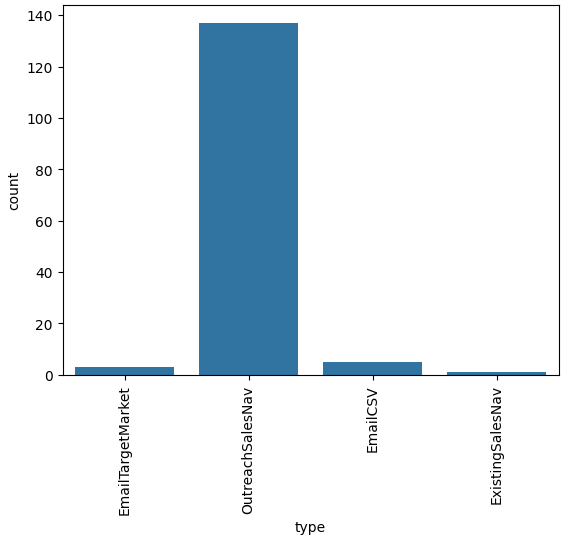
\includegraphics[width=8cm]{src/assets/images/campaign_types.png}}
    \caption{Campaigns by types}
    \label{fig:campaign-types-image}
\end{figure}

The plot above shows that the highest amounts of campaigns is of type `OutreachSalesNav`.
We will only consider that and ignore the rest.

\subsubsection*{Messages by Types}

\begin{figure}[H]
    \centering
    \makebox[\textwidth]{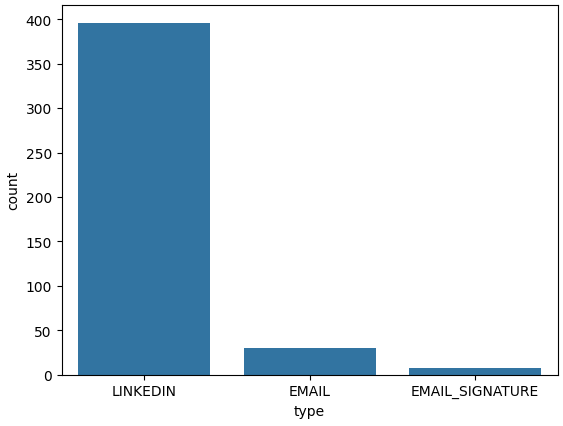
\includegraphics[width=8cm]{src/assets/images/message_types.png}}
    \caption{Messages by types}
    \label{fig:message-types-image}
\end{figure}

The email type messages are for the email campaigns and should be dropped.

The `LinkedIn` type messages are from our `OutreachSalesNav` but some of them can also be from the `ExistingSalesNav`. A cleanup is needed to only keep messages for the campaigns
that are not dropped.

% \subsection{Correlation Analysis}
% tbd

\subsection{Handling Missing Values}

For the leads dataset, the timestamp fields are changed to boolean values.
This is because we are only interested in whether a messages was sent to the lead or not, not when it was sent.

\subsection{Encoding Categorical Variables}

For the leads dataset, we encode the genres with one-hot encoding to make them have the same weight.
As for the other categorical variables, we use label encoding.

\subsection{Feature Engineering}
Seeing that we want to approach this as a Collaborative Filtering problem, we need to create a matrix of users and items.
Or in this case, a matrix of leads and campaign messages.
We will stick with the default name of `users` and `items` to avoid confusion.

\subsection{Target Variable Definition}
The target variable is a list of messages that we want to send to a lead.
For that, we create the unique identifier of the message by concatenating the campaign id and the order of the message in the campaign.

We can then run the Collaborative Filtering algorithm to get the recommendations and map them back to the original messages.

% ----------------------------------- SECTIONS (^) ----------------------------------- %

\setcounter{secnumdepth}{0} % Set the section counter to 0 so next section is not counted in toc
% ----------------------- Conclusion ----------------------- %
\section{Conclusion}
In this chapter, we have presented the datasets that we worked with.
We have also done some data exploration and preprocessing to prepare the data.
For the next chapter where we will talk more about model selection and training.
